The two points relevant to making the game fun according to Sid Meier\todobenjamin{sid meier talk source here} are \textit{Advanced Gameplay} and \textit{Complex Strategical Aspects}, as defined in \ref{sec:specifyingtheproblemstatement}.
Both can be achieved by making a series of interesting decisions.
Sid Meier describes 4 characteristics of interesting decisions: \todomichael{sid meier talk source here}
\begin{itemize}
	\item Trade-offs - Do I buy this big sword, but spend a lot of gold doing so?
	\item Situational - For this track, do I go with the car with good handling or the car with most horsepower?
	\item Personal - Do I build a lot of defensive units and \textit{turtle} \tododaniel{either define turtling or use another word} in my base, or do I play aggressive and try to rush down my enemy?
	\item Persistence - My decisions should be informed and have an impact on the game
\end{itemize}

In order to have the basics of a fun game design, the game's core loop should enable the player to make interesting decisions that affect the game.
Making early prototypes will help to refine the core loop as well as these decisions, especially in regards to giving the right amount of information to the player.
This ties in with the idea of \textit{Cognitive Flow}.

\subsection{Cognitive Flow}
\emph{This section is largely based on an article by Sean Baron, User Experience Researcher at Microsoft Game
Studios\cite{baron}.}

Cognitive Flow is a psychological term for being immersed in a game, or ``in the zone''.
When players are fully immersed in a game, they experience a loss of self-awareness and lose track of time.

To increase the chance of reaching this cognitive flow, four main states in terms of game to player interaction has to
be promoted.  
These four states are 
\begin{itemize}
    \item \emph{Concrete goals with manageable rules}
    \item \emph{Goals that fit player capabilities}
    \item \emph{Clear and timely feedback}
    \item \emph{Removal of distractions from player focus}
\end{itemize}

In order to maximize the fun of the game, these four states must be considered when designing the core game loop, and thus the decisions available to the players.

\subsubsection{Concrete goals with manageable rules}
The player must always know how to accomplish the next goal of their choice, whether it is to get an upgraded weapon, or simply get from A to B.
When players are unaware of what to do next, they are more likely to stop playing.
Following this, it means that reinforcing the players actions by limiting the amount of unnecessary information will keep the player playing for longer.
An example would be animated GUI elements distracting the from combat going on in the game world, or enemies attacking while an NPC is giving an important quest.

\subsubsection{Goals that fit player capabilities}
A game cannot be too easy, nor too hard. 
If the player is in any end of the spectrum, he/she will feel either bored or too stressed.
The sweet point is at just the right balance between the two, as this in fact heightens the performance of the player, see Figure \ref{gamedesign:flowzone}.
\begin{figure}
    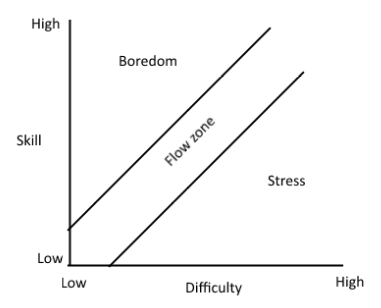
\includegraphics{figures/gamedesign/flowZone}
    \caption{Illustration of the flow zone.}
    \label{gamedesign:flowzone}
\end{figure}

It is important to note that the skill level of a player is highly subjective.
Any new mechanic or game changing feature also has to be taught to the player, if it deviates from the conventional scheme for the genre. 
That is, if the game is a first person shooter, then you do not have to teach the player to aim if it follows the normal conventions, however, if you all of the sudden can jump on walls or walk upside down, then this has to be taught in a setting where teaching is the only focus.

\subsubsection{Clear and timely feedback}
If a player is in doubt about whether he has done something correct, then the feedback timing is off.
If the player shoots a zombie and receives experience points for it, this should happen in a timely manner after zombie has been killed, such that the player can link the reward with the challenge overcome.
Further there has to be short-term mechanisms which convey this information, as well as long-term mechanisms which convey goals spanning longer durations,
such as collecting a key to complete a level, or gathering multiple items to craft a special item.

\subsection{Remove distractions from player focus}
The main focus for the player is for him to be engaged in the game.
If the player has to stop up and pay attention to information, it obstructs gameplay.
Of course there are exceptions to this rule, like giving puzzles which require the player to think in order to solve it.
The trick is making this information precise and concise, such that the information flow from the game to the player is not cluttered with noise and hard to decrypt.
